\documentclass[a4paper,11pt]{article}
\usepackage{graphicx}
\usepackage{float}
\usepackage{subfig}
\usepackage{geometry}
\usepackage{amsmath,amssymb}
\usepackage{amsthm}
\usepackage{bbold}
\usepackage{mathtools}
\usepackage{braket}
\usepackage{booktabs}
\usepackage[table,xcdraw]{xcolor}
\usepackage[utf8]{inputenc}
\usepackage{cite}
\usepackage[english]{babel}
\usepackage{lipsum}
\usepackage{setspace}
%\usepackage{minted}
\usepackage{xcolor}
\newcommand{\R}{\mathbb{R}}
\usepackage{hyperref}
\hypersetup{colorlinks=true,linkcolor=blue}
\geometry{a4paper, top=2.5cm, bottom=2.5cm, left=3cm, right=2.5cm}

\begin{document}
	\author{Catalano Giuseppe, Cerrato Nunzia}
	\title{Numerical Linear Algebra Homework Project 4:\\Unconstrained Optimization}
	\date{}
	\maketitle
	
	In this project we want to perform unconstrained optimization using the Newton method both in its standard form and by considering its variants which make use of the backtracking and the trust region approach. We will apply these methods to four test functions and we will compare these approaches to see how convergence changes.
	
	\section{Algorithms}
	bjdkf bjkfd b
	\section{Test Functions}
	dfbfd
	\subsection*{(a)}
	The first function that we want to consider is the following:
	\begin{equation}
		f(x_{1},x_{2}) = (x_{1}-2)^{4} + (x_{1}-2)^{2}x_{2}^{2} + (x_{2}+1)^{2}.
	\end{equation}
	This function assumes a minimum value, equal to $0$, in the point $(x_{1}^*,x_{2}^*)=(2,-1)$. We would like to obtain this minimum value by using the standard Newton algorithm implemented by the function ****Newton**** in the library ***Project\_4.py ****. We report below the gradient and the Hessian of $f$, which must be passed to the function ****Newton****.
	\begin{equation}
		\nabla f(x_{1},x_{2}) = \begin{bmatrix}
			4(x_{1}-2)^{3} + 2x_{2}^{2}(x_{1}-2)\\
			2x_{2}(x_{1}-2)^{2} + 2x_{2}(x_{2}-2)
		\end{bmatrix},
	\end{equation}

		\begin{equation}
		\nabla^{2} f(x_{1},x_{2}) = \begin{bmatrix}
			12(x_{1}-2)^{2} + 2x_{2}^{2} & 4x_{2}(x_{1}-2)\\
			4x_{2}(x_{1}-2) & 2(x_{1}-2)^{2} + 2
		\end{bmatrix}.
	\end{equation}
	
	\begin{table}
	\centering	
	\begin{tabular}{|c|c|c|c|}
		\hline
		k & $\| \textbf{x}_{k} - \textbf{x}^*\|_{2} $ & $f_{1}(\textbf{x}_{k}) - f_{1}(\textbf{x}^{*}) $ & $-\nabla f_{1}(\textbf{x}_{k})^{T} [\nabla^{2}f_{1}(\textbf{x}_{k})]^{-1} \nabla f_{1}(\textbf{x}_{k})$ \\
		\hline
		0 & $2.236$ & $6.000$ & $-9.000$ \\
		1 & $1.118$ & $1.500$ & $-1.761$ \\
		2 & $6.805\times10^{-1}$ & $4.092\times10^{-1}$ & $ -5.552\times10^{-1} $\\
		3 & $2.592\times10^{-1}$ & $6.489\times10^{-2} $ & $ -1.237\times10^{-1}$ \\
		4 & $5.012\times10^{-2}$ & $2.531\times10^{-3} $ & $ -5.026\times10^{-3}$ \\
		5 & $1.277\times10^{-3}$ & $1.632\times10^{-6}$ & $-3.262\times10^{-6}$ \\
		6 & $1.659\times10^{-6}$ & $2.754\times10^{-12}$ & $-5.508\times10^{-12}$\\
		7 & $1.404\times10^{-12}$ & $1.971\times10^{-24}$ & $-3.943\times10^{-24}$ \\
		\hline
	\end{tabular}
	\caption{Table}
	\label{tab:table_a}
	\end{table}
	
	
	\begin{figure}[H]
		\centering
		\subfloat[][]{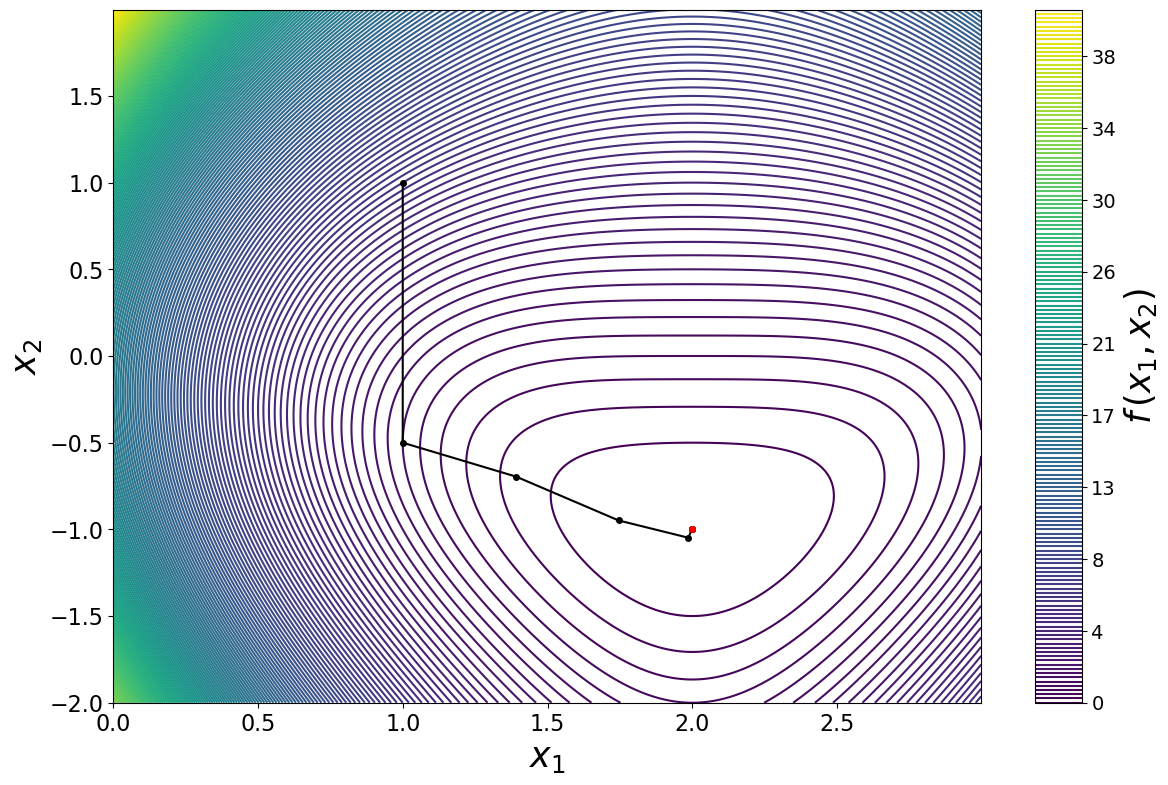
\includegraphics[scale=0.26]{Plot/func_a_standard_newton_contour.png}} \quad
		\subfloat[][]{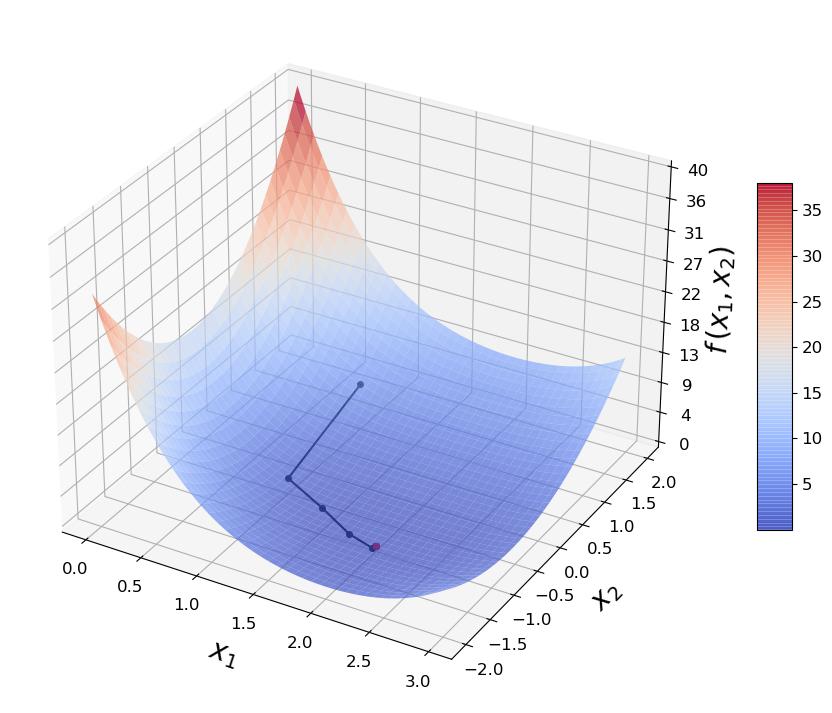
\includegraphics[scale=0.35]{Plot/func_a_standard_newton_3d.png}}
		\caption{Contour plot for the function $f^{(a)}(x_{1},x_{2})$ where the intermediate points are obtained by using the standard Newton method.}
		\label{Fig:func_a}
	\end{figure}

	\subsection{(b)}
	$f:\mathbb{R}^{4} \rightarrow  \mathbb{R}$, $f(\textbf{x}) = \textbf{b}^{T} + \frac{1}{2}\textbf{x}^{T}H\textbf{x}$
	\begin{equation}
		\textbf{b} = (5.04, -59.4, 146.4, -96.6)^{T}
	\end{equation}

	\begin{equation}
		H = \begin{bmatrix}
		0.16 & -1.2 & 2.4 & -1.4 \\
		-1.2 & 12.0 & -27.0 & 16.8 \\
		2.4 & -27.0 & 64.8 & -42.0 \\
		-1.4 & 16.8 & -42.0 & 28.0
		\end{bmatrix}
	\end{equation}

	\begin{table}
		\centering
		\begin{tabular}{|c|c|c|c|}
			\hline
			k & $\| \textbf{x}_{k} - \textbf{x}^*\|_{2} $ & $f_{1}(\textbf{x}_{k}) - f_{1}(\textbf{x}^{*}) $ & $-\nabla f_{1}(\textbf{x}_{k})^{T} [\nabla^{2}f_{1}(\textbf{x}_{k})]^{-1} \nabla f_{1}(\textbf{x}_{k})$ \\
			\hline
			$0$ & $5.745$ & $5.223\times10^{2}$ & $-1.045\times10^{3}$ \\
			$1$ & $9.769\times10^{-13}$ & $2.842\times10^{-14}$ & $-9.948\times10^{-27}$ \\
			$2$ & $1.688\times10^{-13}$ & $0.000$ & $-2.005\times10^{-26}$ \\
			\hline
		\end{tabular}
	\end{table}

	\subsection{(c)}
	$f:\mathbb{R}^{2} \rightarrow  \mathbb{R}$, $f(x_{1},x_{2}) = (1.5 - x_{1}(1-x_{2}))^2 + (2.25 - x_{1}(1-x_{2}^{2}))^2 + (2.625 - x_{1}(1-x_{2}^{3}))^2 $
	
\begin{table}
	\centering
	\begin{tabular}{|c|c|c|c|}
		\hline
		k & $\| \textbf{x}_{k} - \textbf{x}^*\|_{2} $ & $f_{1}(\textbf{x}_{k}) - f_{1}(\textbf{x}^{*}) $ & $-\nabla f_{1}(\textbf{x}_{k})^{T}[\nabla^{2}f_{1}(\textbf{x}_{k})]^{-1} \nabla f_{1}(\textbf{x}_{k})$ \\
		\hline
		$0$ & $5.009$ & $8.17\times10^{1}$ & $-1.455\times10^{2}$ \\
		$1$ & $8.66\times10^{-1}$ & $2.423$ & $-4.527$ \\
		$2$ & $6.494\times10^{-2}$ & $2.407\times10^{-2}$ & $-4.643\times10^{-2}$ \\
		$3$ & $1.393\times10^{-1}$ & $3.45\times10^{-3}$ & $-6.32\times10^{-3}$ \\
		$4$ & $2.103\times10^{-2}$ & $1.383\times10^{-4}$ & $-2.704\times10^{-4}$ \\
		$5$ & $1.377\times10^{-3}$ & $2.863\times10^{-7}$ & $-5.717\times10^{-7}$ \\
		$6$ & $3.033\times10^{-6}$ & $2.186\times10^{-12}$ & $-4.372\times10^{-12}$ \\
		$7$ & $2.836\times10^{-11}$ & $1.233\times10^{-22}$ & $-2.466\times10^{-22}$ \\
		$8$ & $4.441\times10^{-16}$ & $4.437\times10^{-31}$ & $-8.79\times10^{-31}$ \\
		\hline
	\end{tabular}
	\caption{$x_{0}=(8,0.2)^{T}$, backtracking = False}
\end{table}

	\begin{table}
		\centering
		\begin{tabular}{|c|c|c|c|}
			\hline
			k & $\| \textbf{x}_{k} - \textbf{x}^*\|_{2} $ & $f_{1}(\textbf{x}_{k}) - f_{1}(\textbf{x}^{*}) $ & $-\nabla f_{1}(\textbf{x}_{k})^{T}[\nabla^{2}f_{1}(\textbf{x}_{k})]^{-1} \nabla f_{1}(\textbf{x}_{k})$ \\
			\hline
			$0$ & $5.009$ & $2.043$ & $-3.291$ \\
			$1$ & $3.963$ & $2.553\times10^{-1}$ & $-5.885\times10^{-2}$ \\
			$2$ & $4.218$ & $2.328\times10^{-1}$ & $-6.421\times10^{-1}$ \\
			$3$ & $1.661\times10^{1}$ & $5.743\times10^{2}$ & $-9.291\times10^{2}$ \\
			$4$ & $6.137$ & $5.226\times10^{1}$ & $-6.327\times10^{1}$ \\
			$5$ & $3.426$ & $1.596\times10^{1}$ & $-3.709$ \\
			$6$ & $2.974$ & $1.421\times10^{1}$ & $-8.445\times10^{-3}$ \\
			$7$ & $3.041$ & $1.42\times10^{1}$ & $-5.688\times10^{-8}$ \\
			$8$ & $3.041$ & $1.42\times10^{1}$ & $-1.083\times10^{-18}$ \\
			$9$ & $3.041$ & $1.42\times10^{1}$ & $0.000$ \\
			\hline
		\end{tabular}
		\caption{$x_{0}=(8,0.2)^{T}$, backtracking = False *** PROBLEMA? ***}
	\end{table}
	
	
	\begin{table}
		\centering
		\begin{tabular}{|c|c|c|c|}
			\hline
			k & $\| \textbf{x}_{k} - \textbf{x}^*\|_{2} $ & $f_{1}(\textbf{x}_{k}) - f_{1}(\textbf{x}^{*}) $ & $-\nabla f_{1}(\textbf{x}_{k})^{T}[\nabla^{2}f_{1}(\textbf{x}_{k})]^{-1} \nabla f_{1}(\textbf{x}_{k})$ \\
			\hline
			$0$ & $5.009$ & $2.043$ & $-3.291$ \\
			$1$ & $3.963$ & $2.553\times10^{-1}$ & $-5.885\times10^{-2}$ \\
			$2$ & $4.218$ & $2.328\times10^{-1}$ & $-6.421\times10^{-1}$ \\
			$3$ & $2.920$ & $2.131\times10^{-1}$ & $-7.337\times10^{-2}$ \\
			$4$ & $2.471$ & $1.649\times10^{-1}$ & $-1.224\times10^{-1}$ \\
			$5$ & $1.340$ & $1.502\times10^{-1}$ & $-1.22\times10^{-1}$ \\
			$6$ & $1.192$ & $7.989\times10^{-2}$ & $-1.697\times10^{-1}$ \\
			$7$ & $6.453\times10^{-1}$ & $5.012\times10^{-2}$ & $-5.027\times10^{-2}$ \\
			$8$ & $3.335\times10^{-1}$ & $1.73\times10^{-2}$ & $-2.418\times10^{-2}$ \\
			$9$ & $8.357\times10^{-2}$ & $3.009\times10^{-3}$ & $-5.269\times10^{-3}$ \\
			$10$ & $2.128\times10^{-2}$ & $1.004\times10^{-4}$ & $-1.967\times10^{-4}$ \\
			$11$ & $2.767\times10^{-4}$ & $1.503\times10^{-7}$ & $-3.005\times10^{-7}$ \\
			$12$ & $1.103\times10^{-6}$ & $2.293\times10^{-13}$ & $-4.585\times10^{-13}$ \\
			$13$ & $2.404\times10^{-13}$ & $8.166\times10^{-25}$ & $-1.633\times10^{-24}$ \\
			$14$ & $0.000$ & $0.000$ & $0.000$ \\
			\hline
		\end{tabular}
	\caption{$x_{0}=(8,0.2)^{T}$, backtracking = True}
	\end{table}
	
	\begin{figure}[H]
		\centering
		\subfloat[][]{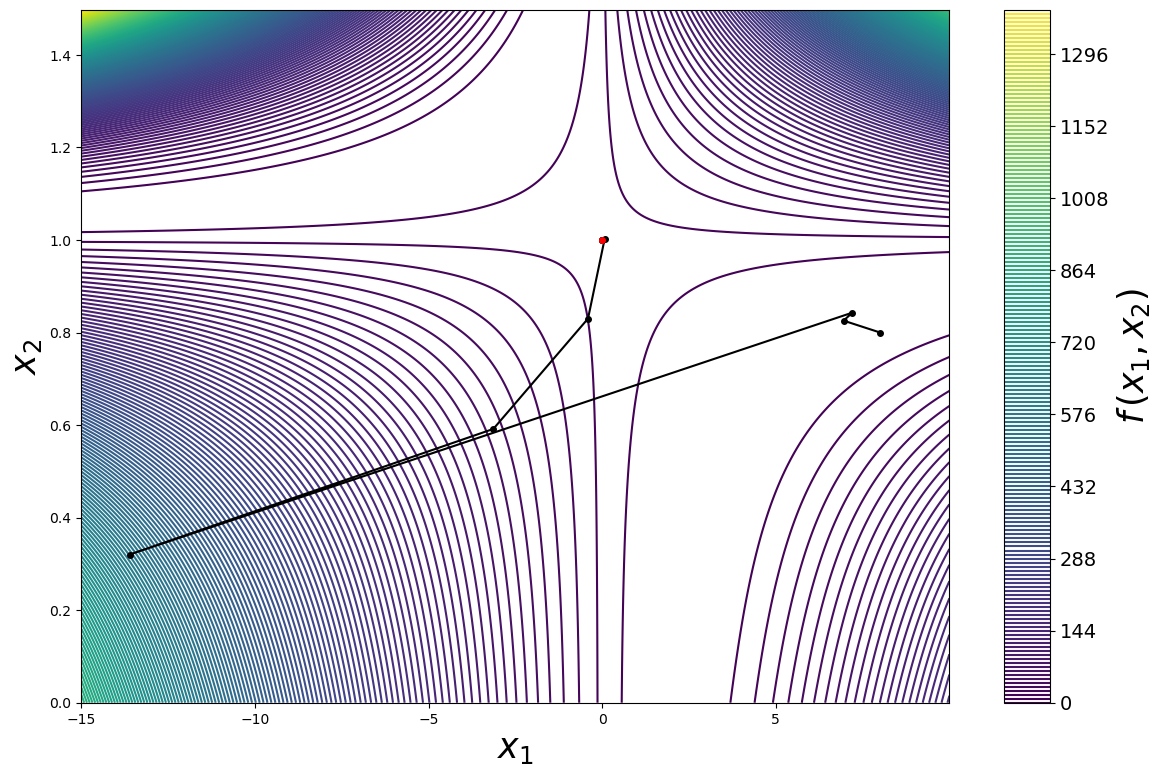
\includegraphics[scale=0.25]{Plot/func_c_standard_newton_contour.png}} \quad
		\subfloat[][]{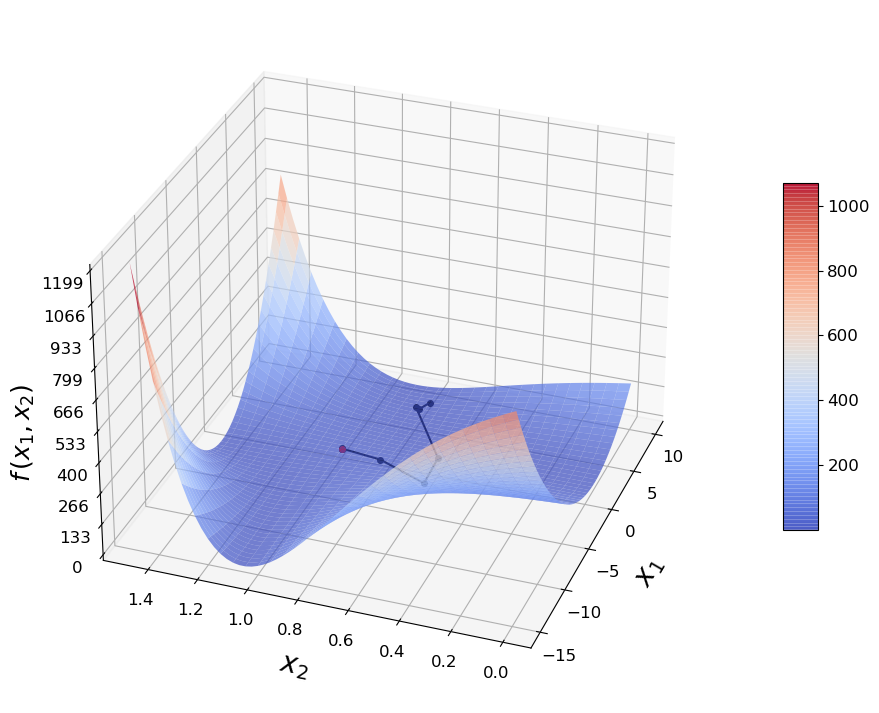
\includegraphics[scale=0.35]{Plot/func_c_standard_newton_3d.png}}
		\caption{Contour plot for the function $f^{(c)}(x_{1},x_{2})$ where the intermediate points are obtained by using the standard Newton method.}
		\label{Fig:func_c}
	\end{figure}

	\subsection{(d)}
	$f:\mathbb{R}^{2} \rightarrow  \mathbb{R}$, $f(x_{1},x_{2}) = x_{1}^{4} + x_{1}x_{2} + (1+x_{2})^{2}$
	
	\begin{table}[H]
		\centering
		\begin{tabular}{|c|c|c|c|}
			\hline
			k & $\| \textbf{x}_{k} - \textbf{x}^*\|_{2} $ & $f_{1}(\textbf{x}_{k}) - f_{1}(\textbf{x}^{*}) $ & $-\nabla f_{1}(\textbf{x}_{k})^{T}[\nabla^{2}f_{1}(\textbf{x}_{k})]^{-1} \nabla f_{1}(\textbf{x}_{k})$ \\
			\hline
			$0$ & $1.119\times10^{-1}$ & $2.385\times10^{-2}$ & $-4.688\times10^{-2}$ \\
			$1$ & $1.209\times10^{-2}$ & $3.79\times10^{-4}$ & $-7.539\times10^{-4}$ \\
			$2$ & $1.264\times10^{-3}$ & $4.365\times10^{-6}$ & $-8.725\times10^{-6}$ \\
			$3$ & $1.272\times10^{-4}$ & $4.4\times10^{-8}$ & $-8.889\times10^{-8}$ \\
			$4$ & $1.272\times10^{-5}$ & $1.649\times10^{-12}$ & $-8.906\times10^{-10}$ \\
			$5$ & $1.271\times10^{-6}$ & $-4.392\times10^{-10}$ & $-8.907\times10^{-12}$ \\
			$6$ & $1.256\times10^{-7}$ & $-4.436\times10^{-10}$ & $-8.907\times10^{-14}$ \\
			\hline
		\end{tabular}
		\caption{$x_{0}=(0.75,-1.25)^{T}$, backtracking = False}
	\end{table}
	
	\begin{figure}[H]
		\centering
		\subfloat[][]{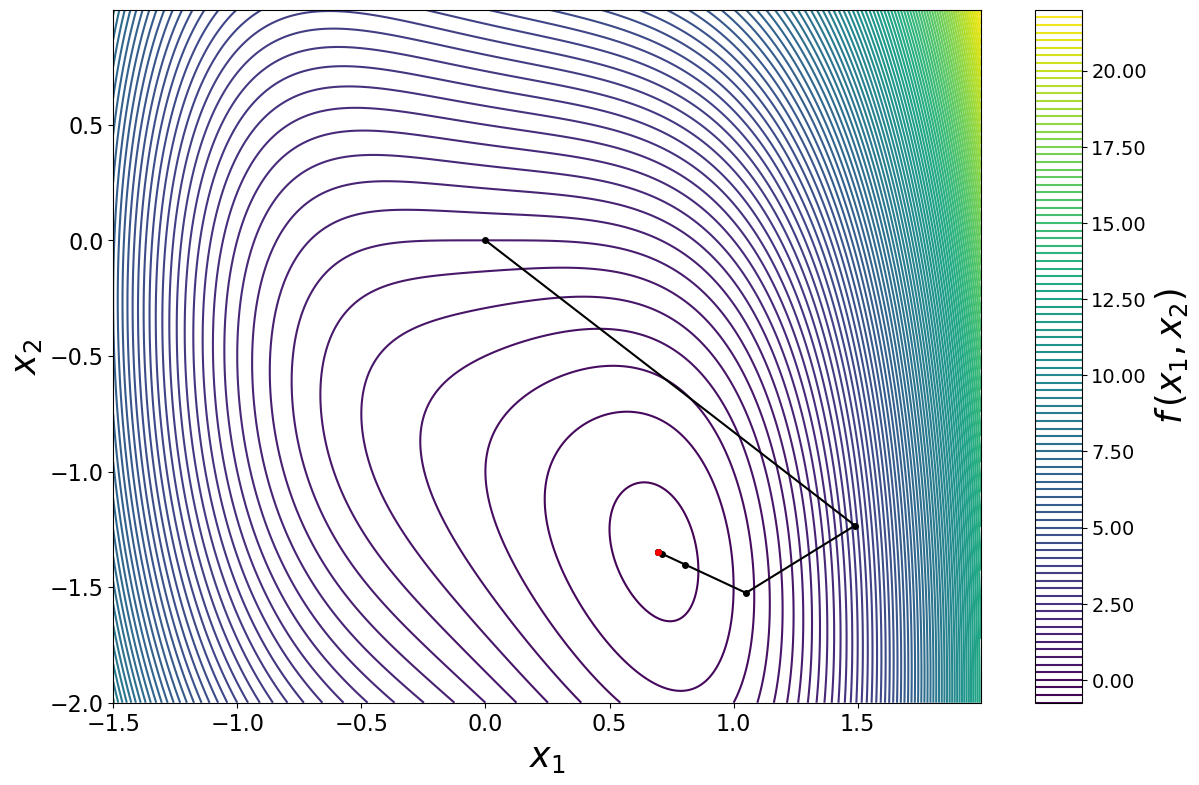
\includegraphics[scale=0.25]{Plot/func_d_newton_trustreg_contour.png}} \quad
		\subfloat[][]{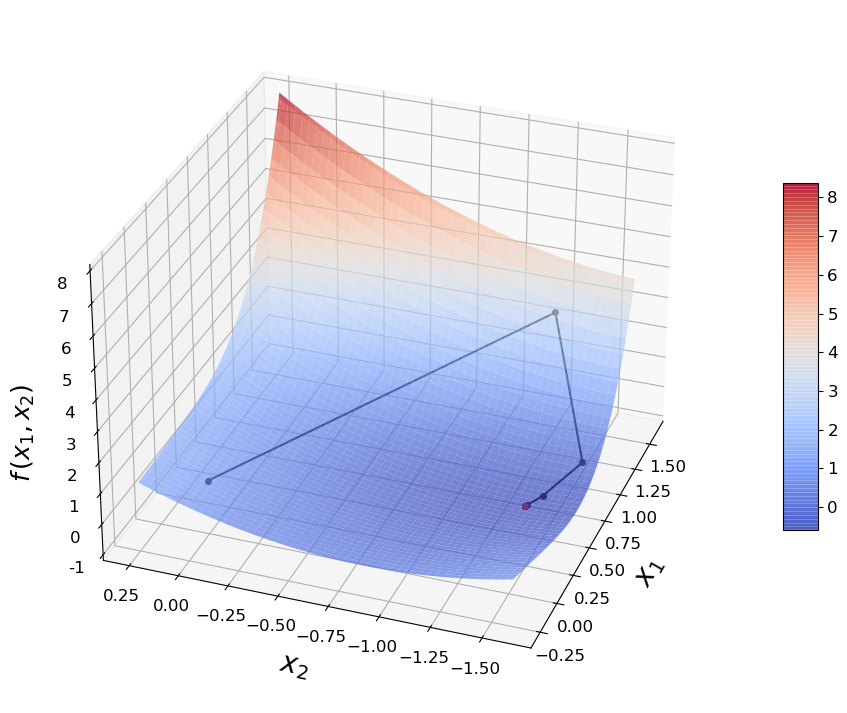
\includegraphics[scale=0.35]{Plot/func_d_newton_trustreg_3d.png}}
		\caption{Contour plot for the function $f^{(d)}(x_{1},x_{2})$ where the intermediate points are obtained by using the standard Newton method.}
		\label{Fig:func_d}
	\end{figure}
\end{document}